\section{Coherently seeded regime: why the output is reproducible}\label{sec:mechanism}

Reservoir computing requires that the same input gives the same output; otherwise a trained readout fails on the next run.
In the single-pump schemes of the literature the comb lines either grow out of noise through modulation
instability~\cite{shishavan2025} or rely on a soliton state prepared beforehand~\cite{cuevas2025,arabieh2026soliton}.
The former's output depends on the noise at start-up; the latter needs the device to be held inside the soliton existence range.
The spectral-phase mask gives a third mode of operation: the input lines themselves sit on resonances and the sidebands are
seeded coherently by the input instead of growing from noise, so the output is set by the input.

\subsection{Two runs compared}

Figure~\ref{fig:two-runs} feeds the same input sequence into the same device twice; the two runs differ only in the initial
intracavity noise. Panel~(a) uses the parameters of the original chaotic-comb scheme (a single CW pump, $325~\mathrm{mW}$, loaded
$Q=10^{7}$, normalised detuning about 5): the power of the third line next to the pump is completely different in the two runs, with
a correlation of only $0.08$; a readout trained on such features gives an NMSE of about 1 on the other run, i.e.\ it learned
nothing. Panel~(b) is an operating point of the spectral-phase mask (the point chosen in the noise-floor study of
Section~\ref{sec:noise}, $23~\mathrm{mW}$, loaded $Q=6\times10^{6}$): the two curves coincide, with correlation $1.00$.

\begin{figure}[htbp]
\centering
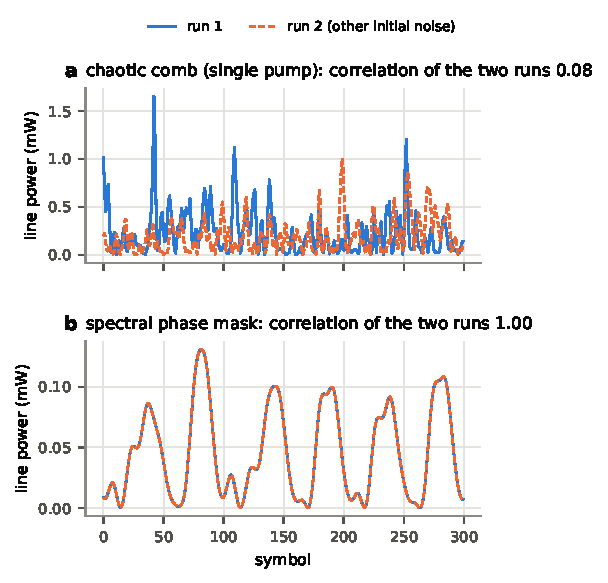
\includegraphics[width=0.8\linewidth]{fig3_two_runs}
\caption{The same input sequence fed into the same device twice; the runs differ only in the initial intracavity noise (solid and
dashed). Shown is the drop-port power of the third line next to the pump over the first 300 symbols.
(a) Parameters of the original chaotic-comb scheme (single CW pump, $325~\mathrm{mW}$, loaded $Q=10^{7}$, normalised detuning
about 5): correlation between the runs $0.08$.
(b) An operating point of the spectral-phase mask ($23~\mathrm{mW}$, loaded $Q=6\times10^{6}$): the curves coincide, correlation
$1.00$. No other noise in either panel.}
\label{fig:two-runs}
\end{figure}

\subsection{Operating map}

Reproducibility holds only in part of the parameter space. Figure~\ref{fig:operating-map} fixes the other parameters of a mask
operating point and scans only the input coupling $\Qone$ ($10^{5.6}$ to $10^{7.6}$) and the total input power ($3$ to
$1000~\mathrm{mW}$) in 17 steps each, plotting the Mackey--Glass test error; for every point we also compute the consistency of
two runs (the correlation between their features).

Without noise the plane splits in two. 74\% of the points have a consistency above $0.99$: the coherently seeded regime.
The inconsistent points (consistency below $0.5$, 16\%) gather in the high-power, high-$Q$ corner (above $163~\mathrm{mW}$), where
the intracavity power lets modulation instability overwhelm the seed and the comb returns to chaos.
The lowest errors lie inside the coherently seeded regime, close to the chaotic one: all points within a factor of three of the
best error ($1.8\times10^{-6}$) fall between $6$ and $79~\mathrm{mW}$ and $\Qone=10^{6.1}$ to $10^{6.85}$. This matches the common
experience in reservoir computing that more nonlinearity helps, but not so much that reproducibility is lost.

Realistic noise adds a third region. At low power many lines reach the detectors with powers comparable to the detector noise,
the readings drown in it, and the consistency drops as well; the share of points with consistency above $0.99$ falls from 74\% to
29\%. The usable operating points are squeezed between the two: limited by detector noise on the low-power side and by chaos on
the high-power side, the points within a factor of three of the best error ($3.3\times10^{-4}$) form a diagonal band in the
power--$Q$ plane ($9$ to $336~\mathrm{mW}$). The higher the $Q$, the less power is needed for the same nonlinearity, so the band
tilts towards lower power as $Q$ increases. The chaotic region is at the same place with and without noise, because its cause
(modulation-instability gain exceeding the seed) does not depend on the noise.

\begin{figure}[htbp]
\centering
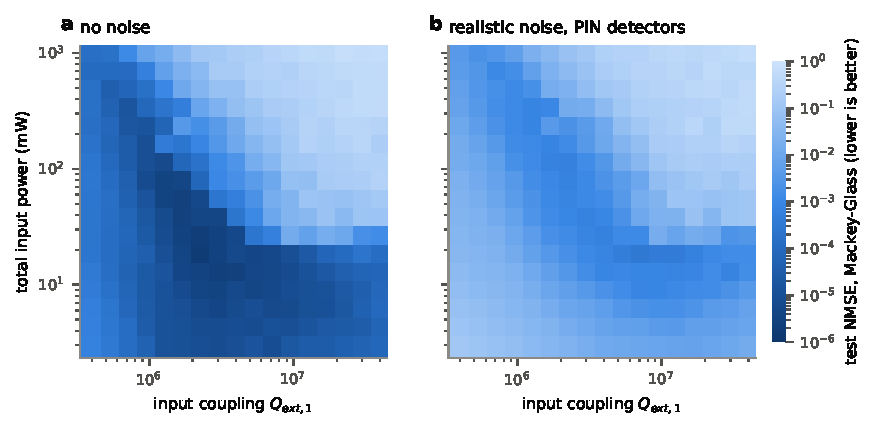
\includegraphics[width=\linewidth]{fig2_operating_map}
\caption{Operating map of the spectral-phase mask. The other parameters of a mask operating point are fixed while the input
coupling $\Qone$ and the total input power are scanned (17 steps each); colour is the Mackey--Glass test error (darker is better).
(a) No noise: the upper right (high power, high $Q$) is the non-reproducible chaotic regime, the rest is coherently seeded, and the
lowest errors lie in the seeded regime close to the chaotic one.
(b) Realistic noise, PIN detectors: the low-power region drowns in detector noise, and the usable points form a band between the
two regions that tilts towards lower power as $Q$ increases. The run-to-run consistency values are given in the text.}
\label{fig:operating-map}
\end{figure}

The conclusion of this section is used throughout the rest of the paper: the spectral-phase mask operates in the coherently seeded
regime, and its error comes from noise, not from non-reproducible dynamics. Lowering the error therefore requires knowing which
noise source is responsible (Section~\ref{sec:noise}).
